\documentclass{bmvc2k}

%% Enter your paper number here for the review copy
%\bmvcreviewcopy{??}

\title{Object-Centric Spatio-Temporal Pyramids for Egocentric Activity Recognition}

% Enter the paper's authors in order
% \addauthor{Name}{email/homepage}{INSTITUTION_CODE}
\addauthor{Tomas McCandless}{tomas@cs.utexas.edu}{1}
\addauthor{Kristen Grauman}{grauman@cs.utexas.edu}{1}

% Enter the institutions
% \addinstitution{Name\\Address}
\addinstitution{
 Department of Computer Science \\ 
 University of Texas at Austin
}

\runninghead{McCandless, Grauman}{Object-Centric Spatio-Temporal Pyramids}

% Any macro definitions you would like to include
% These are not defined in the style file, because they don't begin
% with \bmva, so they might conflict with the user's own macros.
% The \bmvaOneDot macro adds a full stop unless there is one in the
% text already.
\def\eg{\emph{e.g}\bmvaOneDot}
\def\Eg{\emph{E.g}\bmvaOneDot}
\def\etal{\emph{et al}\bmvaOneDot}

%------------------------------------------------------------------------- 
% Document starts here
\begin{document}

\maketitle

\begin{abstract}
	Egocentric video and wearable computing have become increasingly
	prevalent in the past decade, resulting in a huge explosion in the amount
	of available video content and increased attention from the computer
  vision community.
  However, existing methods for activity recognition often use
  predefined spatio-temporal binning schemes
  to aggregate features. This encodes information beyond what is possible
  with a pure ``bag of words'' model, but is ultimately inflexible
  and may fail to capture important spatio-temporal relationships between
  features.
  We propose to randomly generate a pool of candidate binning schemes and
  use a boosting algorithm to select those which are most discriminative for use in our final
  classifier. In order to efficiently focus the candidate partition schemes, we
  create biased partitions using ``object-centric'' cuts in video volumes.
  Partition schemes generated using our method have a high probability of
  cutting through video regions that contain ``active objects,'' the objects
  being interacted with by the user during a given frame.
  Given a set of training vides, our method first computes histograms of
  active object locations across each $(x, y, t)$ dimension, then uses these
  histograms to generate a pool of object-centric partition schemes that
  have a high probability of cutting through regions that often contain
  active objects.
  Next, we represent each training video using each partition scheme and train a pool
	of weak SVM classifiers. 
	Finally, we use a boosting algorithm to learn which partitioning schemes are
  most discriminative and form a
	final strong classifier. Our main novel contribution is two-fold: we show how to learn the
  most useful partition schemes in an egocentric setting, and we focus
  candidate partition schemes by exploiting locations of active objects.
  Our approach yields state-of-the-art recognition performance, and we find
  that object-centric partition schemes are often more discriminative than
  their unbiased counterparts.
  % TODO closing statement
\end{abstract}

%------------------------------------------------------------------------- 
\section{Introduction}
  % uses for egocentric activity
  % recent research without detailed explanation
	Activity recognition is becoming an increasingly canonical problem in
	computer vision as researchers are beginning to explore the domain more
  thoroughly and several relevant datasets have been released 
  \cite{Schuldt04, Rodriguez08, Fathi11, Ramanan12}. 
  Egocentric activity recognition differs from
  non-egocentric activity recognition because activities can have long-term
  temporal dependencies and actions can be interrupted by other actions. 
	% application to life logging
	A robust and accurate method for egocentric activity recognition would have 
	useful practical applications, such as a memory aid, content-based
  summarization, or telerehabilitation. For instance,
	a recent trend in wearable computing is so-called life logging which can
	assist patients suffering from memory loss \cite{Sellen07}. 
	A robust egocentric activity recognition
	system could automatically tag video clips with types of activities.
  Additionally, there are many clinical benchmarks used to evaluate patients everyday
  functional abilities \cite{Kopp97, Catz97, Itzkovich07}. 
  These benchmarks are currently conducted in a
  hospital setting, but a robust system for egocentric activity
  recognition
  could greatly impact the workflow for patient evaluation, allowing
  for passive long term observation of patients in their own
  homes.
  Existing work has made promising progress in both recognition and
  summarization, \cite{Ramanan12, Fathi12,Lee12} 
  yet it remains a challenging problem.






  % egocentric defined by objects, binning with preservation of object
  % relationships is unclear.
  % existing work uses hand coding
  % cite ramanan, choi, laptev but not in detail
  Egocentric activities
  are well-defined by the types of objects that are interacted with by users
  during particular actions (``active objects'') \cite{Ramanan12}, yet how to optimally aggregate
  features across space-time remains unclear.
  The familiar bag-of-words approach can be used to aggregate 
  features with reasonable performance, but ultimately falls short because it
  fails to capture temporal dependencies between features.
  The pyramid is a well-known extension of a pure bag-of-words model that encodes spatial
  relationships between features by recursively subdividing images or video and extracting 
  features from each spatial bin \cite{Lazebnik06}, yielding impressive
  results across a range of applications.
  Existing methods for activity recognition often rely on
  hand-coded partition schemes \cite{Ramanan12, Choi08, Laptev08}.
  With a small pool of hand-coded schemes for imposing spatial
  information, the most discriminative space-time relationships between features may not be 
  captured. 
% it is problematic to use hand-coded partitions because...







  % our idea: learn partitions
  Our idea is to randomly generate a pool
  of candidate partitioning schemes. 
  We then aggregate spatio-temporal features in a
  learned way, using a boosting algorithm to select those partitioning schemes which are most discriminative.
  % focus the partition generation
  Boosting is computationally expensive in terms of the number of weak
  classifiers that are used, and there are many high-dimensional
  partitioning schemes we could sample. This suggests that a large pool of
  candidate partition schemes is required to obtain good performance.
  In order to avoid generation of partitions that are not discriminative, we
  introduce object-centric partitioning schemes, which have a high
  probability of cutting through video regions known to contain active
  objects.
  





  % method overview short, mention partition generation and boosting
  Given a set of labeled training videos with object annotations (bounding boxes and
  active/passive tags), our method first computes histograms of active
  object locations across each $(x,y,t)$ dimension of video. We use these
  histograms to generate a pool of object-centric partition schemes that have a high
  probability of cutting through regions known to frequently contain active
  objects. We compute feature vector representations of each training video clip using each
  candidate in the pool, and use these vectors to train a pool of weak SVM
  classifiers. Finally, we use a boosting algorithm to select the partitions
  which are most discriminative and form a final strong classifier.






  % results teaser -- not just improvement on stoa, but detail on what will
  % be shown
  We find that object-centric partitioning schemes that have a larger number
  of levels are often the most discriminative in the sense that they tend to
  get selected by boosting over their unbiased counterparts.
  We evaluate the performance of our method using a cross-validation
  experiment and find that our method using object-centric pyramids improves
  upon the current state of the art.





	

%-------------------------------------------------------------------------
\subsection{Related Work}

  %--------
  % activity recognition in general




  % BoW methods for video (laptev, choi, ramanan)






  % egocentric analysis: recognition, summarization.
  % yong jae, lu zheng, fathi/ren (and some of their refs)
  % main point: importance of objects in egocentric vs other cues in other
  % domains





  % spatial binning strategies
  % kovashka, lazebnik, sharma, jiang (but not too much credit to jiang)











  The work presented in \cite{Kovashka10}
  describes an effective state-of-the-art method for learning the shapes of spatio-temporal
  regions on a per-class basis, but makes use of lower-level features such as
  optical flow, rather than object locations, and
  is not applied in an egocentric setting.
  Spatial pooling of features in a learned way for object recognition in 2D images
  has been thoroughly
  explored \cite{Sharma11}, but to our knowledge there has been little work
  on learning the best way to pool spatio-temporal features in video.

	In \cite{Laptev08}, Laptev \etal investigate automatically aligning movie scripts with
	video for the purpose of annotating human actions, and achieve 91.8\%
  accuracy on the KTH dataset. 
  Previous work on spatial pyramids \cite{Bosch07, Lazebnik06} is
  extended
  by defining the spatio-temporal pyramid representation of video clips, but uses a
  relatively small number of predefined schemes for spatio-temporal binning,
  which may fail to capture important spatio-temporal relationships between
  features. There are 6 possible spatial grids and 4 temporal binning
  schemes, resulting in a total of 24 possible spatio-temporal partition
  schemes. 
	
	In \cite{Marszalek09}, Marszalek \etal released a novel dataset based on
	Hollywood movies that contains twelve types of activities and ten
	different classes of scenes. The main contribution of this paper is based
	on the observation that the visual content of a human's environment can
	impose useful constraints on the type of activity occurring. For instance,
	food preparation activities frequently occur in a kitchen environment. 
	
	In \cite{Fathi12}, Fathi \etal focus on the relationship between gaze and
	activity recognition in an egocentric setting and develop methods to
	predict activity given gaze, gaze given activity, and both
	activity and gaze given neither. The activities in this
	published dataset are primarily related to food preparation. 
	
	The main work related to our own is that carried out in \cite{Ramanan12}. 
	In this work the ADL dataset is introduced as well as detailed analysis of
	performance of several different classifiers. 
	\begin{figure}[t]
		\begin{center}
			%\fbox{\rule{0pt}{2in} \rule{0.9\linewidth}{0pt}}
			  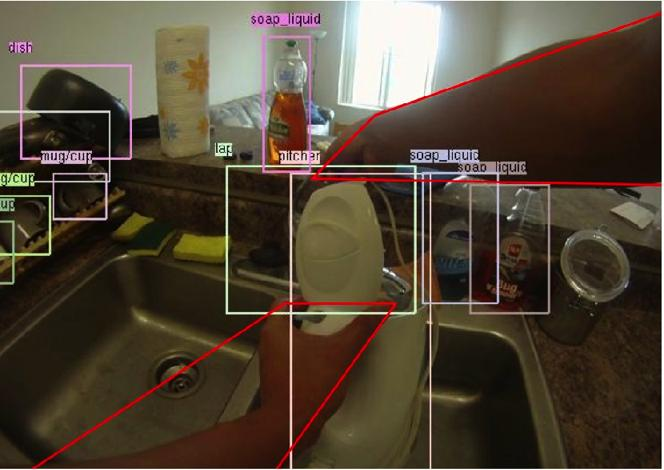
\includegraphics[width=0.7\linewidth]{figures/thumbnail.jpg}
		\end{center}
    \caption{An example frame from the ADL dataset with annotations for hand
    position and detected objects} 
				\label{fig:long}
				\label{fig:onecol}
	\end{figure}
  Composite object models are developed for the purpose of object detection. 
  These models take advantage of the fact that objects can have vastly
  different appearances when they are being interacted with. For example, a
  refrigerator or microwave has a different appearance when it is open and
  being interacted with. 
  A comparison of the well-known bag-of-words approach with a strict
  predefined
  2-level temporal pyramid using both space-time interest points and the
  results of the part-based object detectors is presented. The temporal pyramid makes 
  a single cut along the temporal dimension and no cuts along the
  spatial dimensions, but is simple, easy to implement, and outperforms a 
  classifier trained on bag-of-words histograms. The use of detected objects as
  features offers impressive improvement over using space-time interest points
  (STIP).
	The crucial contribution of
	\cite{Ramanan12} is that egocentric activity recognition is ``all about
	the objects'', particularly the objects being interacted with, as
	recognition accuracy increases dramatically when locations of active
  objects in addition to passive objects are used as features. 

	The video collected for the ADL dataset is available in a temporally
	presegmented format; each video has been segmented into clips depicting
	activities. Egocentric video is captured as a continuous stream, and thus
  a pre-processing step of temporal segmentation into discrete events is
  required. There is a large amount of literature on temporal segmentation
  of video. For instance, work presented in \cite{Lee12} includes a method for
	automatic temporal segmentation of egocentric video into events.
  
	Our algorithm is inspired by the work of \cite{Jiang12}, which uses a
  a version of the SAMME Ada-boost algorithm \cite{Zhu06}
  with randomized spatial pyramids for 2D images, 
	leading to increased robustness to intra-class variation based on results
  from benchmarks on three publicly available datasets. However, in contrast
  to our own work, the randomized pyramids are not biased in any way. 
	
	% work from other researchers on segmentation
	% work from other researchers on activity recognition with other modes of
	% sensor data

\section{Approach}

	Our boosting algorithm takes as input a collection of labeled training videos
	and a pool of candidate partition patterns. We use the output of the
  aforementioned object detectors trained on composite object models as our features to be
  pooled.
  We train a separate ``weak''
  multi-class SVM 
  (using LIBSVM \cite{Chang11})
	classifier on the feature vectors resulting from representing the training
	data using each candidate partition pattern $\theta$. We set a weight
  $w_i$ for each
	training point $p_i$ that is inversely proportional to the number of points
	with the same class as $p_i$. Giving larger weights to training examples of
  infrequently occurring actions helps to mitigate any bias resulting from imbalanced
  training data.
  During each round of boosting we select the
	candidate partition $\theta_j$ that is most discriminative (has minimum
  weighted training
	error, which is computed as the dot product between the weight vector $w$
  and an indicator of incorrect classifications using $f_\theta$)
  Next, we compute a weight for $\theta_j$, and compute accuracy for the
	current version of the final strong classifier, which maximizes a weighted
  sum of classifications produced by each weak classifier.
	We set the number of boosting rounds to 30.\\

	\noindent\textbf{Algorithm 1:} Training RSTP Classifier via Boosting \\
	\textbf{INPUT:} 
	\begin{itemize}
		\item $N$ labeled training videos $\Phi = \{(V_i, c_i)\}_{i=1}^N$
		\item A pool of $M$ partition patterns $\Theta = \{\theta\}$
	\end{itemize}
	\textbf{OUTPUT:}
	\begin{itemize}
		\item A strong video classifier $F$. For an unlabeled video $V$, 
			$c=F(V)$ is the predicted label for $V$.
	\end{itemize}
			\begin{enumerate}

				\item For each $\theta \in \Theta$:
					\begin{itemize}
            \item Compute the representations of each $V_i \in \Phi$ using $\theta$
						and train a multi-class classifier (SVM) $f_\theta$ on the
            resulting feature vectors.
					\end{itemize}

				\item Initialize:
					\begin{itemize}
						\item A weight $w_i = \frac{1}{C N_{c_i}}$ for each video clip,
							where $N_{c_i}$ is the number of videos with label $c_i$,
              and $C$ is the number of distinct labels in the training data.
						\item Current iteration number $j=0$.
						\item Current accuracy $\sigma_j = 0$.
					\end{itemize}

				\item For each round of boosting:
					\begin{itemize}
						\item Increment $j$.
						\item Re-normalize the weight vector:
              \begin{center}
              $\forall i, w_i = \frac{w_i}{\Sigma_i^N w_i}$.
              \end{center}
					  \item For each pattern $\theta$,
              compute its weighted classification error:
              \begin{center}
              $e_\theta = w \cdot \mbox{\textbf{I}}(f_\theta(V) \neq c)$
              \end{center}
						\item Choose the pattern $\theta_j$ with minimum weighted
              classification error $e_j$.
						\item Compute the weight for $\theta_j$:
              \begin{center}
              $\alpha_j = \mbox{log} \frac{1 - e_j}{e_j} + \mbox{log}(C-1)$
              \end{center}
						\item Update the weight vector:
              \begin{center}
							$w_i = w_i \cdot \mbox{exp}(\alpha_j \cdot
							\mbox{\textbf{I}}(f_{\theta_j}(V_i) \neq c_i))$.
              \end{center}
						\item Generate the current strong classifier:
              \begin{center}
							$F(V) = \mbox{argmax}_c \Sigma_{m=1}^j \alpha_m \cdot
							\mbox{\textbf{I}}(f_{\theta_m}(V) = c)$
              \end{center}
					\end{itemize}

			\end{enumerate}
	

  \subsection{Generating Randomized Spatio-Temporal Partitions (RSTP)}
  An RSTP is generated using a hierarchical partitioning of feature space.  
  We generate cuts independently in a round-robin manner over dimensions $(x, y, t)$. 
  Each cut is axis-aligned
  (we incorporate random shifts, but not random rotations).
  To construct a partition scheme that is easily applicable to videos of
  arbitrary size, we consider
  partitioning an ``idealized'' video clip that has all dimensions normalized
  to length 1. To generate a single cut we sample a random number from a
  uniform distribution subject to any constraints imposed by ``parent cuts'' and use
  this as a randomized offset for an appropriate axis-aligned plane. To
  construct an unbiased partition scheme we sample from a uniform
  distribution.
  
  To represent a video clip as a randomized spatio-temporal pyramid (RSTP)
  using a particular partition scheme we use the output of object detectors
  trained in \cite{Ramanan12}, which gives bounding boxes and object
  labels for each extracted frame. We use centroids of bounding boxes to
  obtain $(x,y,t)$ coordinates for each individual object.
  We compute histograms of detected
  objects for each individual level in the pyramid,
  where level 0 is the entire video clip volume and level $i$ is all the
  cells of depth $i$ in the k-d tree. 
  Note that level $i$ has $8^i$ leaf
  cells. To form the final RSTP representation, we concatenate the
  histograms computed for each level to form a single feature vector.
  We can choose whether or not to include detected active objects when
  forming an RSTP representation of a video clip, however taking active
  objects into account gives a substantial improvement to overall
  classification accuracy.
  
  \subsection{Generating Object-Centric Cuts (OCC)}
  There are many high-dimensional partition schemes that we could sample
  randomly, which suggests that a very large pool of candidate partition
  schemes is required to obtain good results. However, boosting is
  computationally expensive, so we would like to minimize the size of the
  pool while maintaining good results.
  One of the main contributions of our work is the ability to generate
  meaningfully biased randomized partition schemes that tend to be more discriminative
  than their unbiased counterparts.
  To accomplish this, we propose to replace the uniform distribution with a discrete
  approximation of the distribution of active objects across each dimension
  $(x, y, t)$
  and otherwise proceed normally.

\begin{figure}
  \begin{center}
\begin{tabular}{cc}
\bmvaHangBox{\fbox{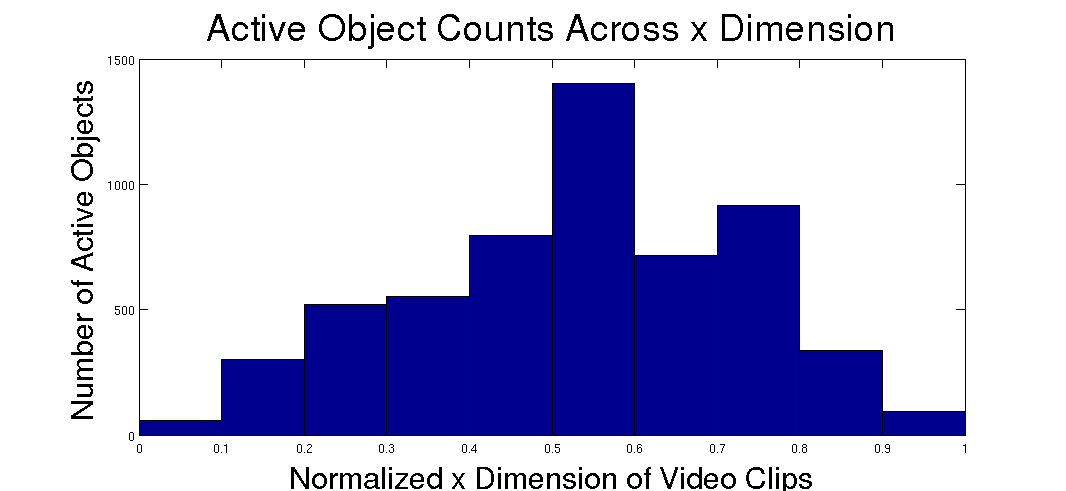
\includegraphics[width=5.9cm]{figures/active_obj_distr_x.png}}}&
\bmvaHangBox{\fbox{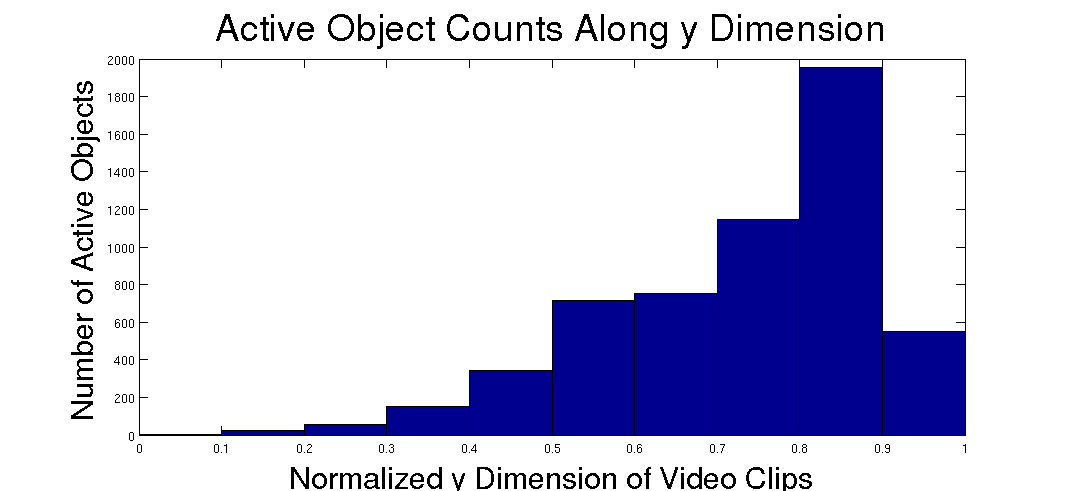
\includegraphics[width=5.9cm]{figures/active_obj_distr_y.png}}}\\
(a)&(b)
\end{tabular}
		   \caption{Histograms of detected active objects across the $x$ and
       $y$ spatial dimensions of training data. Active objects tend to appear in the lower
     center field of view. There is a slight bias favoring the
   right side of the field of view because many users are right-handed. }
\label{fig:teaser}
  \end{center}
\end{figure}
	
	From figure 2 we see that active objects often tend to occur in the lower center
	of the field of view. This conforms to our expectations, because
	the active objects are close to the hands which are in the lower field of
	view from an egocentric perspective. Active objects tend to occur on the
  right side of the field of view slightly more often because a large
  percentage of users are right-handed.
  The distribution of active objects
  across the temporal dimension is nearly uniform. 
  Since different clips can have
  varying lengths with respect to time, we normalize the length of each
  video clip to 1 and consider relative temporal locations of active
  objects. 
	For biased partitions, we generate
  the first split along each dimension according to a weighted distribution
  corresponding to the histograms of observed active object regions in the training data,
  and we generate all subsequent child cuts using a uniform distribution.
  We do not consider locations of passive objects at all during the
  generation of biased partition schemes. Since active objects are located
  in close spatial proximity to hands, creating biased partition schemes can
  be interpreted as implicitly taking into account information about hand
  locations.
  
  Figure 3 depicts an example 3-level object-centric partition scheme. 
  The salient feature to note is that visible splits along the $y$
  dimension correspond to the observed distribution of active objects along
  the $y$ dimension of the training data.

\section{Results}
  The ADL dataset consists of hundreds of egocentric video clips
	(roughly 10 hours of video in total) collected from 20 people performing
	18 types of unscripted actions in their own homes. These naturally
  occurring
  actions are often related to hygiene or food preparation and are more
  varied than actions presented in previous datasets such as that of \cite{Fathi11}.
  There are 26 different 
	types of detected objects, including 5 active and 21 passive objects. 
  Object detectors are trained on videos from the
  first 6 people and tested on the videos from the remaining 14 people.
  
	\begin{table}
		\begin{center}
			\begin{tabular}{|l|c|}
				\hline \hline
        label & activity type \\
        \hline
        1 & combing hair \\
        \hline
        2 & make up \\
        \hline
        3 & brushing teeth \\
        \hline
        4 & dental floss \\
        \hline
        5 & washing hands/face \\
        \hline
        6 & drying hands/face \\
        \hline
        7 & laundry \\
        \hline
        8 & washing dishes \\
        \hline
        9 & moving dishes \\
        \hline
       10 & making tea \\
        \hline
       11 & making coffee \\
        \hline
       12 & drinking water/bottle \\
        \hline
       13 & drinking water/tap \\
        \hline
       14 & preparing cold food/snack \\
        \hline
       15 & vacuuming \\
        \hline
       16 & watching tv \\
        \hline
       17 & using computer \\
        \hline
       18 & using cell phone \\
				\hline
			\end{tabular}
		\end{center}
		\caption{Types of activities present in the ADL dataset.}
	\end{table}
  
	Each frame in the dataset
	is annotated with activity labels and bounding boxes for detected objects and hand positions, 
	Additionally, each object is tagged as active or passive depending
	on whether it is being interacted with.
	The ADL dataset has been modified since the publication of
	\cite{Ramanan12}; because of this, running the published code gives
	slightly lower accuracy than the originally published numbers. We use the
  modified version of the dataset available from the authors webpage at the time of writing to
  benchmark our method. One difficulty that can arise within egocentric
  activity recognition is that activities can be temporarily interrupted by
  other activities. For instance, while waiting for tea to brew a subject
  may watch TV. For cases of such interruptions, to avoid unnecessary
  complications resulting from frames being annotated with multiple
  activities, the ADL dataset simply uses the label of the interrupting
  action when a longer action is disrupted.
	
  
  \subsection{Action Recognition Performance}
  Following \cite{Ramanan12}, we evaluate recognition performance on the ADL
  dataset using a form of cross
	validation (the video clips from person $i$ are used as a held out validation set, and
	training occurs using the video clips from the remaining people).
  We exclude videos from the first 6 people
  (because they were used to train the object detectors) from our
  experiments.
  The results for the bag of words baseline and temporal pyramids (2 level, with
  a single cut along the temporal dimension) are both presented in
  \cite{Ramanan12}.
  

	  Table 2 shows a comparison of overall classification accuracy between our
  approach and the method based on temporal pyramids which is
  presented in \cite{Ramanan12}. The temporal pyramid
  has two levels, formed by making a single cut along the temporal
  dimension and no cuts along the spatial dimensions.
  Row 1 shows results
  obtained using only passive detected objects, while row 2 shows results obtained
  using both active (being interacted with) and passive detected objects.
  The consideration of active objects when constructing feature vectors
  gives a significant improvement over just including passive objects, and
  in both cases our method improves on the current state of the art.

  \begin{table}
		\begin{center}
			\begin{tabular}{|l|c|c|c|c|c|}
				\hline
        Feature Type & BoW & Temporal Pyramid \cite{Ramanan12} & RSTP & RSTP+OCC \\
				\hline\hline
        O & 26.6\% & 29.0\% & 35.4\% & 32.7\%\\
        \hline
        AO & 34.9\% & 36.9\% & 33.7\% & 38.7\%\\
				\hline
			\end{tabular}
		\end{center}
		\caption{Overall classification accuracy on pre-segmented video clips,
    evaluated using a form of cross validation. Our boosted classifiers
  improve on the current state of the art.}
	\end{table}
  
	For this experiment we used pools of 4-level partitioning schemes of
  varying sizes with a varying number of boosting rounds. The numbers
  presented in Table 2 were obtained with 5 boosting rounds and a pool of
  size 70.
  The work of \cite{Jiang12}, which uses a similar
  pyramid-based boosting approach for 2D image recognition, found that using
  pyramids with more than 3 levels actually led to a decrease in overall
  accuracy due to over-segmentation of image space. However, we found that in the
  3D case 4-level pyramids give better overall accuracy than coarser-grained
  representations.


  
  \begin{figure}
  \begin{center}
  \bmvaHangBox{\fbox{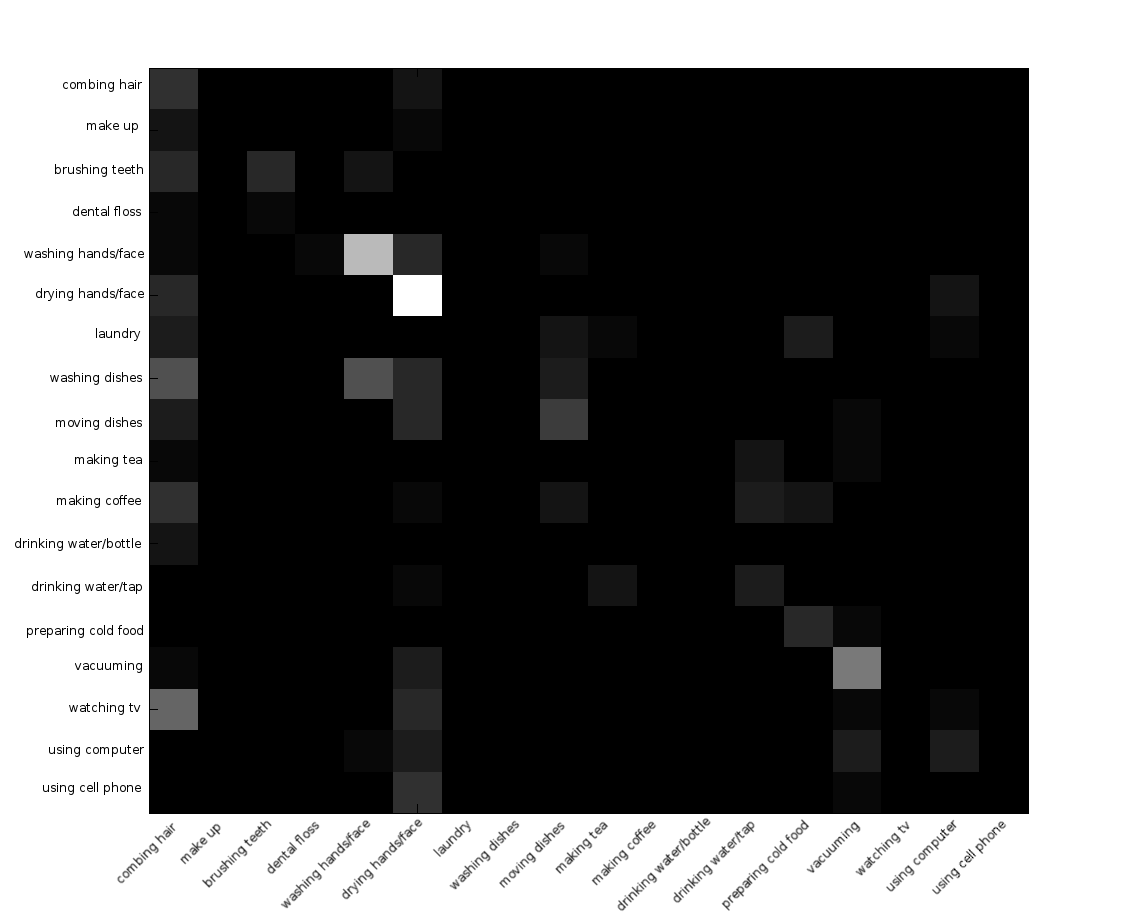
\includegraphics[width=10.0cm]{figures/confn2-labels.png}}}
		   \caption{Confusion matrix for RSTP+OCC using detected active and
       passive objects}
  \label{fig:teaser}
  \end{center}
  \end{figure}
 	As seen in Figure 3, our method has particularly good
  performance for activity types 5 and 6 (``combing hair'' and ``drying
  hands/face'', respectively). Some activity types on which our method does
  poorly are 10 and 11, which are ``making tea'' and ``making coffee'',
  respectively (see Table 1 for a full listing of activity types present in
  the ADL dataset). Since the two activity types are similar in the sense that
  they involve the same active objects, it is not
  unexpected that a recognition system would confuse them often.
   
  \subsection{Effect of Object-Centric Partition Schemes}
	

  To illustrate the improvement on accuracy obtained from using a pool of
  biased partitions, we created separate pools containing 4-level
  partition schemes of each bias type and
  repeatedly ran the cross-validation experiment, adding additional
  partitions to each pool between runs. The pool containing object-centric partitions 
  consistently outperformed the unbiased pool.
  The
  results from this experiment are depicted in figure 4. We were initially
  surprised to find that increasing pool size can
  sometimes negatively impact overall classification accuracy, however we
  believe this is due to the inherent bias between the training and the test
  data. In other words, sometimes a partition scheme with small training error
  on the train data that gets selected during a round of boosting can have a
  larger training error on the test data. 
 
  \begin{figure}[t]
		\begin{center}
			%\fbox{\rule{0pt}{2in} \rule{0.9\linewidth}{0pt}}
			  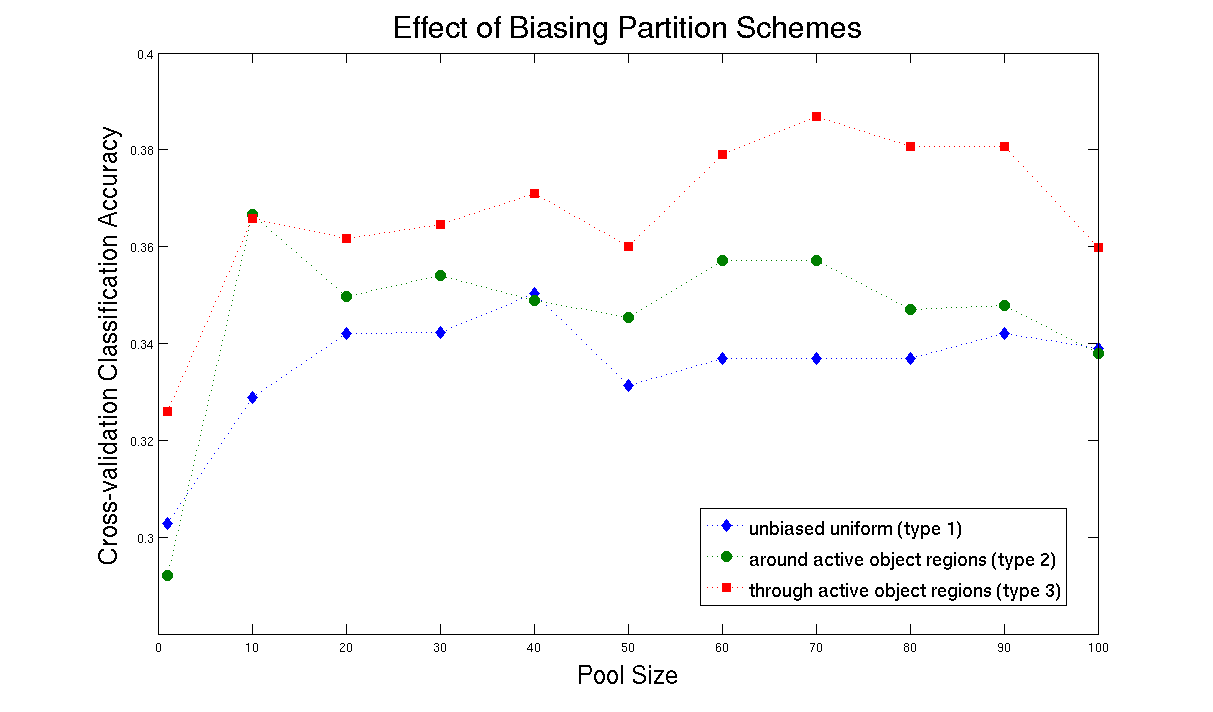
\includegraphics[width=1.0\linewidth]{figures/biaseffect.png}
		\end{center}
		   \caption{Effect of using biased partition schemes. The pool
       containing type 3 biased partition schemes consistently outperforms
     the other pools.}
				\label{fig:long}
				\label{fig:onecol}
	\end{figure}
  
  \subsection{Analysis of Selected Partitions}
  To further support our claim that 4-level pyramids of bias type 3 tend to be most
  discriminative, we created a heterogeneous pool containing partition
  schemes of
  several different types. Specifically, the heterogeneous pool contains 30 2-level
  partitions of each bias type, 30 3-level partitions of each bias type, and
  30 4-level partitions of each bias type, for a total of 270 partitions.
  We generated 20 random 50/50 train/test splits, fixed the number of
  boosting rounds to 5, and observed which types of partitions were most
  often selected during boosting rounds.
  We found that partition schemes with more levels tend to get selected more
  often during boosting rounds.
  Specifically, we found that 2-level pyramids of bias type 3 were selected
  21\% of the time, 3-level pyramids of bias type 3 were selected 19\% of
  the time, and 4-level pyramids of bias type 3 were selected 37\% of the
  time. 2-level and 4-level unbiased pyramids were never selected. Thus,
  biased partition schemes that cut through regions that tend to contain
  active objects are clearly more discriminative than other types of
  partition schemes, especially those which are unbiased.
	
\section{Conclusion and Future Work}
	Our main novel contribution is two-fold. We show how to learn the most
  discriminative partition schemes for spatio-temporal binning in video feature space, and
  we introduce object-centric partition schemes, which have a high
  probability of cutting through video regions known to frequently contain
  active objects. Unlike previous work, we randomly generate a pool of
  candidate partitioning schemes and select those which are most
  discriminative using a boosting algorithm.
  Our recognition approach improves on the current state of the art, and our
  experiments demonstrate the positive impact of taking active object
  locations into account by generating object-centric partition schemes.
  
  In future work, we intend to investigate ways of learning the most
  discriminative partition schemes on a per-class basis.
	Additionally, it may be possible to incorporate different types of biases when generating
	partitions. The ADL dataset also includes annotations for hand positions,
	which we have incorporated implicitly through our generation of
  object-centric cuts.
	However,
	it could be possible to incorporate explicit information given by hand
	positions to obtain better results.
	The partitions we focus on contain cuts that are
  planar and axis-aligned (we consider random shifts but not random
  rotations, and we do not consider non-planar splits),
  but it is possible to carve up the
	video volume in more advanced non-linear ways. Such a method would 
  make histogram computation more expensive	, but may yield a more discriminative
	partitioning scheme that could lead to better classification accuracy.
\bibliography{egbib}
\end{document}
